\documentclass{article}
\usepackage[utf8]{inputenc}
\usepackage{authblk}
\usepackage{setspace}
\usepackage[margin=1.25in]{geometry}
\usepackage{graphicx}
\graphicspath{ {./figures/} }
\usepackage{subcaption}
\usepackage{amsmath}
\usepackage{animate}
\usepackage{hyperref}

\usepackage{lineno}
% \linenumbers
%%%%%% Bibliography %%%%%%
% Replace "sample" in the \addbibresource line below with the name of your .bib file.
% \usepackage[style=nejm, 
% citestyle=numeric-comp,
% sorting=none]{biblatex}

%%%%%% Title %%%%%%
% Full titles can be a maximum of 100 characters, including spaces. 
% Title Format: Use title case, capitalizing the first letter of each word, except for certain small words, such as articles and short prepositions
\title{Inferencia de Matrices de Contacto a partir de datos demográficos utilizando Machine Learning}

%%%%%% Authors %%%%%%
% Authors should be listed in order of contribution to the paper, by first name, then middle initial (if any), followed by last name.
% Authors should be listed in the order in which they will appear in the published version if the manuscript is accepted. 
% Use an asterisk (*) to identify the corresponding author, and be sure to include that person’s e-mail address. Use symbols (in this order: †, ‡, §, ||, ¶, #, ††, ‡‡, etc.) for author notes, such as present addresses, “These authors contributed equally to this work” notations, and similar information.
% You can include group authors, but please include a list of the actual authors (the group members) in the Supplementary Materials.
\author[1]{Lia Zerquera Ferrer}
\author[1]{Daniel C\'ardenas Cabrera}
\author[1]{Javier Oramas L\'opez}
\author[1]{Darío Fragas González}
\author[1]{Dianelys Cruz Mengana}
\author[1]{Mauricio Mahmud Sánchez}
\author[1]{Sergio Pérez Pantoja}
%%%%%% Affiliations %%%%%%
\affil[1]{Facultad de Matem\'atica y Computaci\'on de la Universidad de La Habana}
% \affil[2]{Department of Astronomy, B University, City, Country.}
% \affil[*]{Address correspondence to: email@email.c\usepackage{animate}
% \affil[$\dag$]{These authors contributed equally to this work.}

%%%%%% Date %%%%%%
% Date is optional
\date{}

%%%%%% Spacing %%%%%%
% Use paragraph spacing of 1.5 or 2 (for double spacing, use command \doublespacing)
\onehalfspacing

\begin{document}

\maketitle

%%%%%% Abstract %%%%%%
\begin{abstract}
    En este trabajo inferimos matrices de contacto a partir de datos demográficos usando técnicas de Aprendizaje de Maquina(Machine Learning). Describimos el proceso de recogida de datos y las adaptaciones hechas a los mismos para hacer mas fácil su uso atendiendo a nuestras necesidades. Haciendo uso de estos datos creamos poblaciones y brindamos una implementación de una simulación sobre dichas poblaciones para obtener matrices de contacto. Una vez que tenemos un dataset lo suficientemente grande entrenamos varias arquitecturas de redes neuronales y hacemos una comparación de los sus resultados de estas en la tarea de inferir matrices de contacto.
\end{abstract}

\section{Estado del Arte}

Los modelos matemáticos han desempeñado un papel clave en la comprensión de la propagación de enfermedades infecciosas de transmisión directa, como la Enfermedad del Coronavirus 2019 (COVID-19), así como en la efectividad de las respuestas de salud pública. Dado que el riesgo de contraer infecciones de transmisión directa depende de las interacciones entre las personas, los modelos matemáticos suelen utilizar matrices de contacto para caracterizar la propagación de los patógenos infecciosos. Estas matrices de contacto suelen generarse a partir de encuestas basadas en diarios de contactos. Sin embargo, la mayoría de los lugares en el mundo no cuentan con estudios de contacto empíricos representativos, por lo que se han construido matrices de contacto sintéticas utilizando datos de encuestas específicas del entorno disponibles sobre la composición de hogares, escuelas, aulas y lugares de trabajo.\\
En el estado del arte podemos observar dos enfoques principales, uno de ellos generar poblaciones sintéticas a partir de características demográficas que simulan el comportamiento de la población\'on y a partir de eso obtienen la matriz\cite{socialcontacts}. Una de las grandes desventajas de este enfoque es el costo computacional que trae consigo. Otro de los enfoque es usar solamente modelos estadísticos como la modelización jerárquica bayesiana\cite{projectic-contacts}

\section{Matriz de Contacto}
Una matriz de contacto de una población es una representación de las interacciones o contactos entre los individuos de esa población. En el contexto de la epidemiología, por ejemplo, una matriz de contacto puede mostrar cómo las personas interactúan entre sí y potencialmente transmiten enfermedades.

La matriz de contacto es una estructura bidimensional que suele representarse como una tabla o una matriz numérica. En esta matriz, las filas y las columnas corresponden a los individuos de la población, y cada elemento de la matriz indica la frecuencia o la intensidad del contacto entre dos individuos específicos.

Las matrices de contacto son de gran importancia a la hora de modelar y simular enfermedades infecciosas, ya que proporcionan información sobre cómo se propagan las enfermedades dentro de una población. Estas matrices pueden utilizarse como insumo para modelos epidemiológicos que ayudan a comprender la dinámica de la propagación de enfermedades y a evaluar estrategias de control y prevención.

\section{Propuesta}
La solución propuesta por este artículo es generar una población a partir de datos demográficos y hacer microsimulaciones para simular el comportamiento de la población y de ahí obtener la matriz de contacto asociada a esa población.\\
A partir de los datos demográficos y la matriz de contacto obtenida mediante la simulación se puede crear un dataset para entrenar modelos de aprendizaje de maquinas que sean capaz de inferir a partir de datos demográficos la matriz de contacto sin realizar el costoso proceso de construcción de la población y ejecutar las simulaciones.\\ 
El objetivo de este enfoque es obtener resultados equivalentes a la simulación en un menor tiempo, factor crítico a la hora de tomar decisiones en momentos de crísis.

\section{Construcci\'on del dataset}
En este estudio se utilizaron principalmente los datos demográficos de Cuba extraídos del anuario estadístico de Cuba del 2020\cite{anuario} y el Censo Nacional de Población y Vivienda del 2012 \cite{censo}.

Los datos seleccionados para la construcción de la población fueron:\\

\begin{tabular}{*{3}{|c}|}
\hline
Población por provincias & Población total & \% empleo/desempleo \\
\hline 
\% personas en edad laboral & \% hombres trabajando & \% mujeres trabajando \\
\hline 
Escuelas (por tipo) por mil hab. & Universidades por provincia & grupos de edad \\
\hline
Distribución por grupos de edad & Distribución hombre/mujer & Barrios por 1000 hab. \\
\hline 
Cantidad de personas por casa & total de estudiantes & distribución por tipo de escuela \\
\hline
\end{tabular}\\

Una vez que obtenidos los datos se crea una población a la cual se le asignan edad, hogar, barrio, centro trabajo o escuela, sexo y familia de acuerdo a las respectivas distribuciones de probabilidad. Una vez hecho esto se guarda la población con sus datos en base datos.\\

Fue necesario utilizar un sistema de bases de datos dado que el costo en memoria de crear una población de 12 millones de personas superaba los 50 GB.

\subsection*{Detalles de la simulación } 
Una vez que está creada la poblaci\'on solo es necesario representar las instituciones o lugares por los cuales se va a mover dicha población, estos lugares se representan mediante un grafo de la siguiente manera:

\begin{figure}[h]
        \centering
        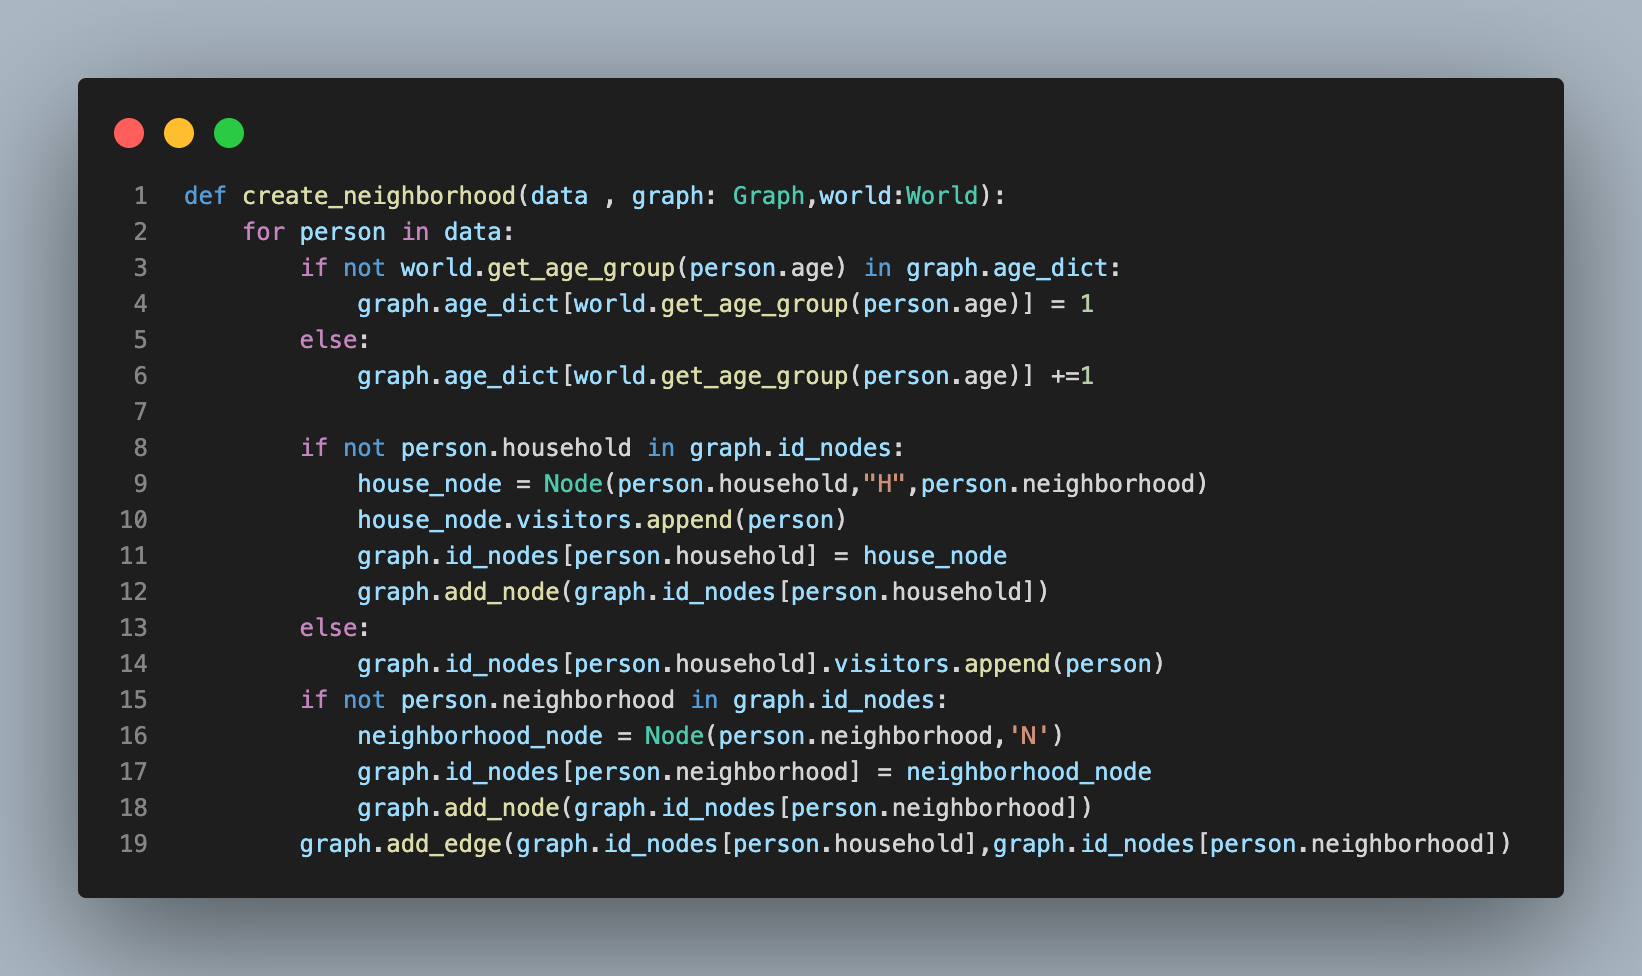
\includegraphics[width=0.8\textwidth]{neighborhood.png}
        \centering
        \caption{Creación de los nodos casas y vecindario del grafo}
    \end{figure}
\begin{itemize}
    \item Primero se crean las casas, para ello se itera por cada persona de la población si la casa a la que esta asignada si esta creada se conecta mediante una arista al vecindario correspondiente a la persona en caso contrario se crea ese nodo casa y se conecta al vecindario que le corresponde si ya existe dicho vecindario, en caso contrario se crea el nodo vecindario y se conecta. \textbf{Figure 1}.
    \item Luego se crean los nodos escuela y trabajo, el procedimiento es similar, se itera por las personas en caso de trabajar/estudiar si no existe aún se crea el nodo escuela/trabajo y se conecta con el nodo casa correspondiente a la persona, en caso de existir ya el nodo escuela/trabajo simplemente se conecta \textbf{Figure 2}.
    \item Adem\'as se crean los nodos que representan lugares de entretenimiento y se conectan de forma aleatoria a alguno de los lugares ya existentes en el grafo.
    \item Por ultimo se crean arbitrariamente nuevas conexiones entre algunos nodos, para brindar una mayor movilidad de la población. 
\end{itemize}

\newpage

\begin{figure}[h]
        \centering
        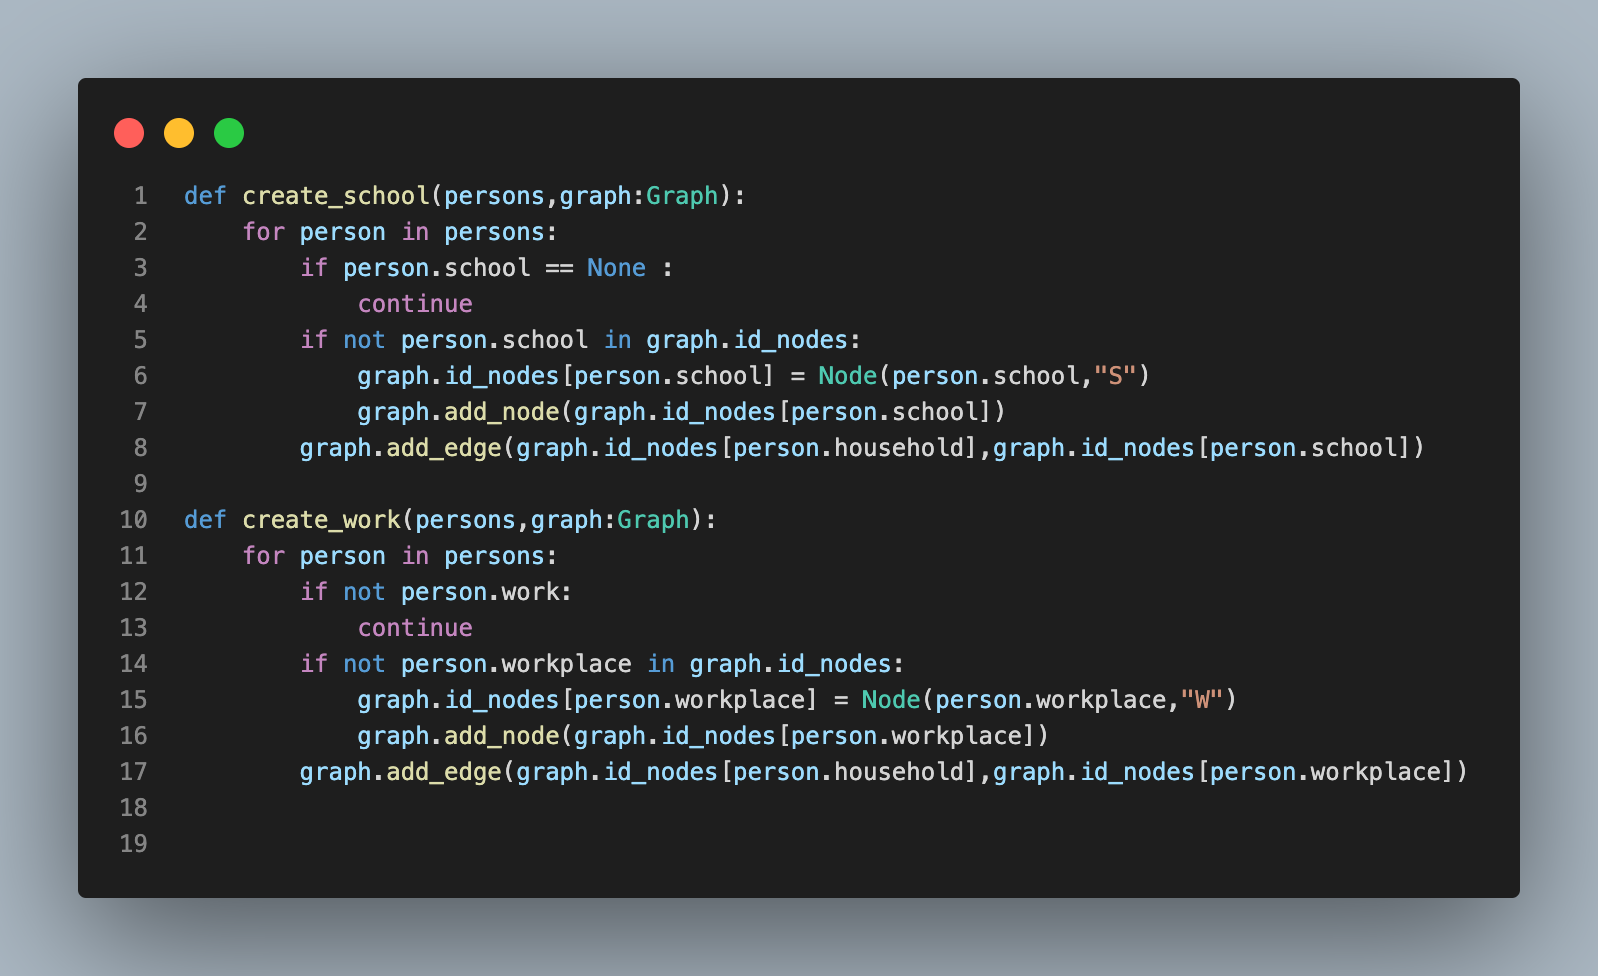
\includegraphics[width=0.8\textwidth, height=0.3\textheight]{school_work.png}
        \centering
        \caption{Creación de los nodos escuela y trabajo}
    \end{figure}

\begin{figure}[h]
  \centering
  \animategraphics[width=\textwidth, height=0.3\textheight, autoplay, loop, framerate=1]{1}{graph/image}{1}{10}
  \caption{Representación gráfica de la creación del grafo}
\end{figure} 

\newpage

Una vez construido el grafo y la población es momento de correr la simulación, inicialmente en la simulación todos las personas de la población se encuentran es sus hogares, luego se itera por cada persona y en dependencia del lugar en donde se encuentre y su rol en la sociedad se realiza una distribución de probabilidad que representar\'a la probabilidad de moverse a los lugares adyacentes al nodo donde se encuentra; luego atendiendo a esta distribución de probabilidad se obtiene el nodo al que se mueve la persona y se actualiza su posici\'on, se realiza este proceso con todas las personas de la población y una vez que se termine se informa el fin de un paso de la simulación \textbf{Figure 4}.\\
\begin{figure}[h]
        \centering
        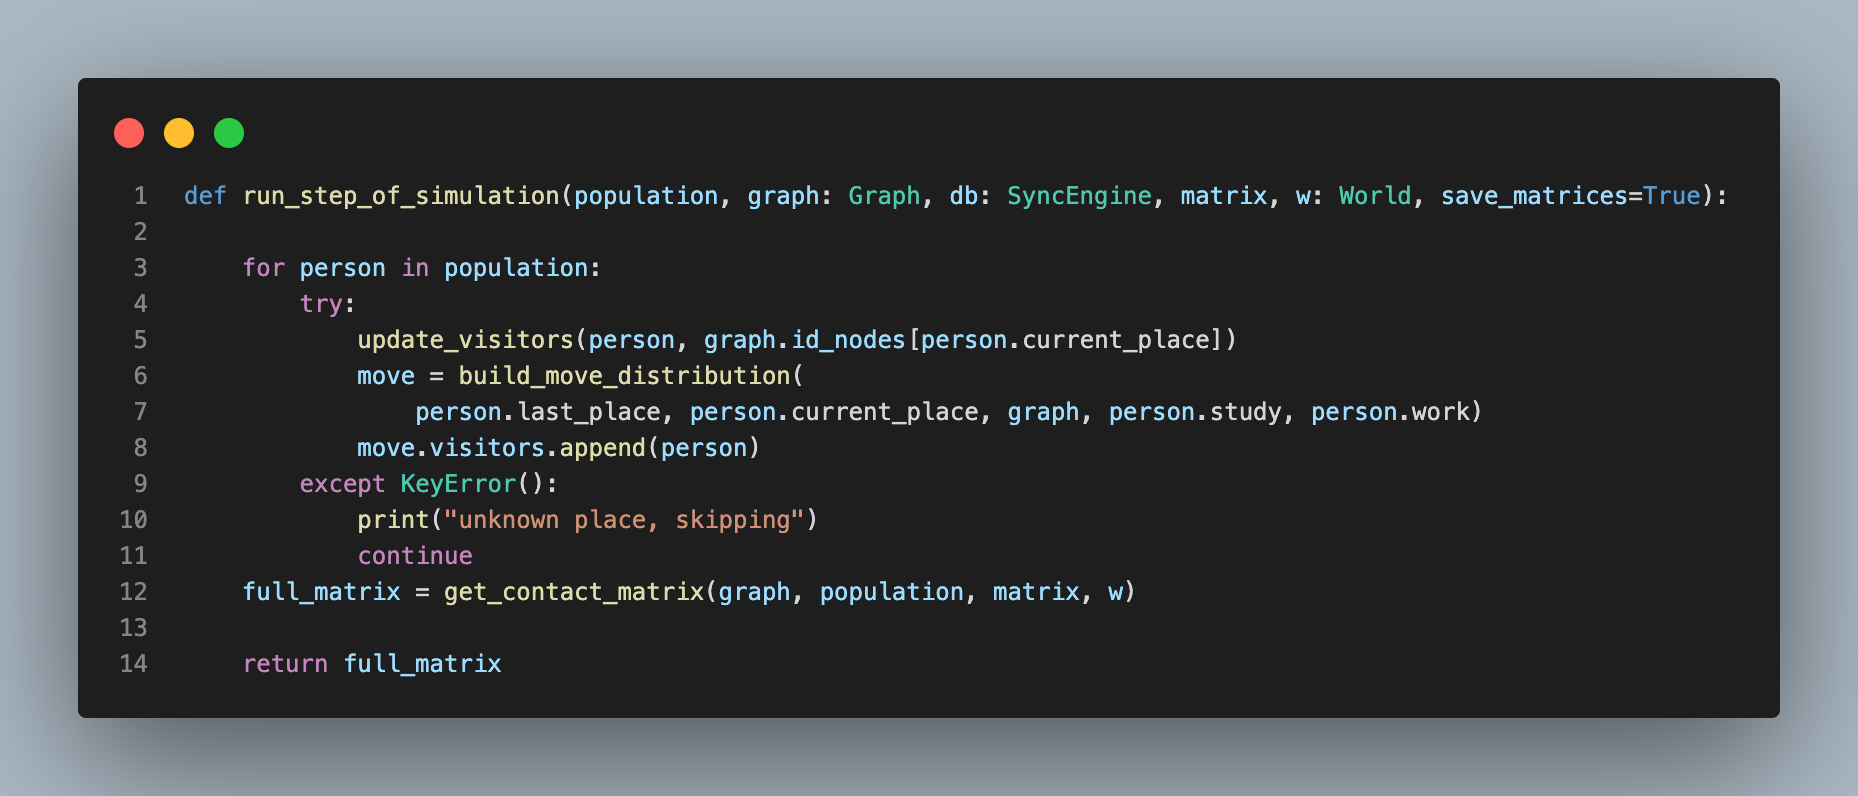
\includegraphics[width=0.8\textwidth,height=0.3\textheight]{step_of_simulation.png}
        \centering
        \caption{Paso de la simulación}
    \end{figure}

Luego de cada paso se halla la matriz de contacto, para ello se recorre cada nodo del grafo y teniendo en cuenta los visitantes de cada nodo y el tipo de nodo se van actualizando la cantidad de contactos de los rangos de edad.\\
En este estudio se decide realizar 10 pasos de simulación por cada población, ya durante el proceso de experimentación se notó que luego de varias iteraciones el comportamiento de la población tendía a tener poca variación.\\
Una vez terminados los 10 pasos de la simulación se normaliza la matriz y se guarda en base datos, junto con los datos demográficos vectorizados \textbf{Figure 5}.


\begin{figure}[h]
        \centering
        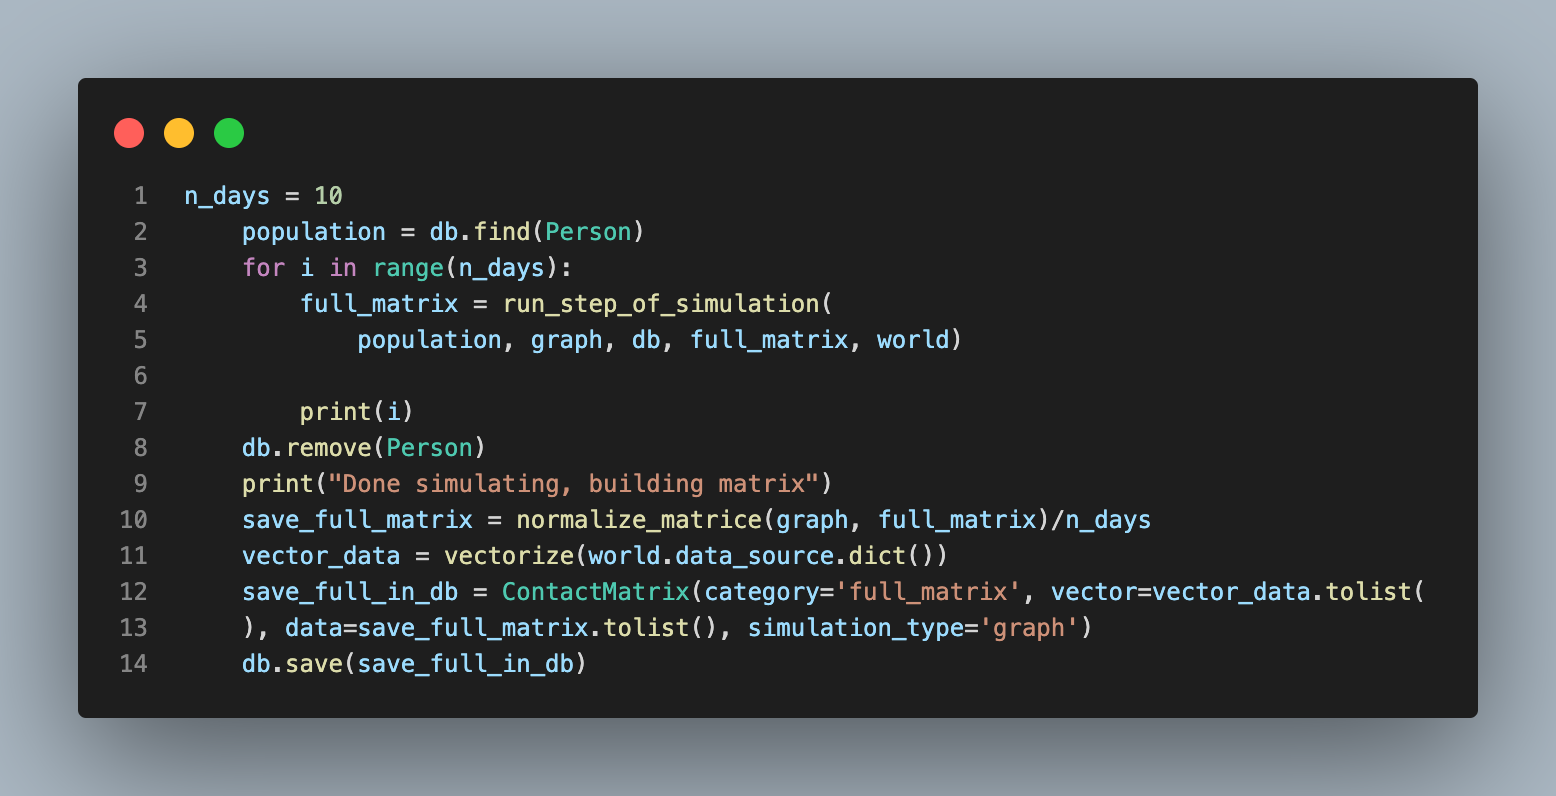
\includegraphics[height=0.3\textheight, width=0.8\textwidth]{run_simulation.png}
        \centering
        \caption{Correr la simulación}
\end{figure}

\vspace{1.5cm}

\section{Técnicas de ML probadas }
\subsection{Red Neuronal}
Las \textbf{redes neuronales artificiales} (también conocidas como sistemas conexionistas) son un modelo computacional evolucionado a partir de diversas aportaciones científicas que están registradas en la historia\cite{5}. Consiste en un conjunto de unidades, llamadas neuronas artificiales, conectadas entre sí para transmitirse señales. La información de entrada atraviesa la red neuronal (donde se somete a diversas operaciones) produciendo unos valores de salida.\\
Se utilizaron con fines de experimentación 2 de los tipos clásicos de redes neuronales, Artificiales, Recurrentes (ANN,RNN).

\subsubsection*{Como recibe el dataset}
En todos los casos se reciben los datos de entrada como un vector de 128 dimensiones que es el resultado de convertir los datos demográficos a vector.

En el caso de las ANN y RNN los datos de salida se representan como un vector de 196 dimensiones que es el resultado de aplanar la matriz de contactos generada por la simulación.

\subsubsection*{Descripción de las redes}
La ANN se diseñó con 7 capas densas con 256, 512 y 1024 neuronas.\\
La RNN de una capa densa, hace un reshape para pasar a una capa TimeDistributed englobando una capa densa y de ahí pasa a una capa LSTM de la cual se obtine el vector de salida.
Ambas redes con optimizador adam y métrica de pérdida "mse".

\subsection{AutoML con Autokeras}
\subsubsection*{Como recibe el dataset}
El dataset se empaqueta en un Dataset de tensorflow y estos datos se pasan directamente al AutoModel de keras.
Nuevamente se utiliza la matriz de contacto aplanada.

\subsubsection{Descripción del modelo}
Se utilizaron tanto el AutoModel como el StructuredDataRegressor ambos con inputs con un StructuredDataInput 
haciendo una exploración del espacio de soluciones utilizando como métrica mse e intentando un máximo de 100 soluciones 


\section{Resultados}
En general los resultados no son alentadores, la poca correlación de la matriz de contacto con los datos en bruto se hace notar.
A continuación se representan en una tabla los resultados de algunas de las métricas obtenidas de cada enfoque.\\


    \begin{tabular}{*{4}{|c}|}
        \hline
        Model &  mean squared error & mean absolute error & median absolute error  \\
         \hline
         ANN & 74.31 & 0.29 & 0.21 \\ 
         \hline
         RNN & 74.39 & 0.14 & 0.09\\ 
         \hline
         AutoModel (autokeras) & 75.03 & 0.3 & 0.23 \\ 
         \hline
         StructuredDataRegressor (autokeras) & 74.69 & 0.06 & 0.003\\ 
         \hline 
    \end{tabular}
\\
Se puede observar una consistencia entre los modelos, aparentando la imposibilidad de aprender más de los datos con los que se cuenta. Esto nos hace pensar que tal vez la simulación no sea lo suficientemente buena o que aplicar redes neuronales, en esta tarea no es el mejor enfoque.

\section{Recomendaciones}
El proceso de simulación es considerablemente lento, por lo cual, por razones de tiempo se tuvo que parar la generación de ejemplos de entrada dejando un dataset de 1411 elementos, se recomendaría seguir este enfoque y generar una cantidad superior.

Introducir en el modelo protocolos que cambien el orden de los individuos, esto en particular se puede hacer modificando el diccionario politics-deployed de la clase World que define la posibilidad (en porciento) de moverse hacia un lugar u otro, además de implementar algún ente que decida en que momento modificar estos parámetros.\\

Probar con otras bibliotecas de AutoMl, se intentó ejecutar con AutoGOAL pero no se logró configurar de manera correcta y, nuevamente, por razones de tiempo, se descartó. 
\begin{thebibliography}{99}
\bibitem{projectic-contacts} Projecting contact matrices in 177 geographical regions: an update and comparison
with empirical data for the COVID-19 era
\bibitem{socialcontacts} Inferring the Structure of Social Contacts from Demographic Data in the Analysis of Infectious Diseases Spread.
\bibitem{anuario} Anuario Estadístico de Cuba 2020, Edición de 2021 -  \href{http://www.onei.gob.cu/node/18491}{ONEI}
\bibitem{censo} Censo de Población y Viviendas 2012, Edición de 2014
- 
\href{http://www.onei.gob.cu/sites/default/files/informe_nacional_censo_0.rar}{ONEI}
\bibitem{5} \href{http://www.itnuevolaredo.edu.mx/takeyas/apuntes/Inteligencia%20Artificial/Apuntes/tareas_alumnos/RNA/Redes%20Neuronales2.pdf }{Historia de las redes neuronales pdf}


\end{thebibliography}

\end{document}
